\documentclass[12pt,a4paper,oneside]{scrarticle}

\usepackage
[
        a4paper,% other options: a3paper, a5paper, etc
        left=25mm,
        right=15mm,
        top=20mm,
        bottom=20mm,
]
{geometry}
\usepackage{setspace}
\setstretch{1.5}


%---------Russian-----------
\usepackage[T2A]{fontenc}
\usepackage[utf8]{inputenc}
\usepackage[russian]{babel}
%---------Russian-----------

%---------Graphics-----------
\usepackage{graphicx}
\graphicspath{{./img}}

\usepackage{tikz}
%---------Graphics-----------

%---------Chemistry-----------
\usepackage{chemfig}
%---------Chemistry-----------

%---------Title-----------
%\title{Работа}
%---------Title-----------

\begin{document}
\section{Поиск компонент связности}

\begin{figure}[h]
	\centering
	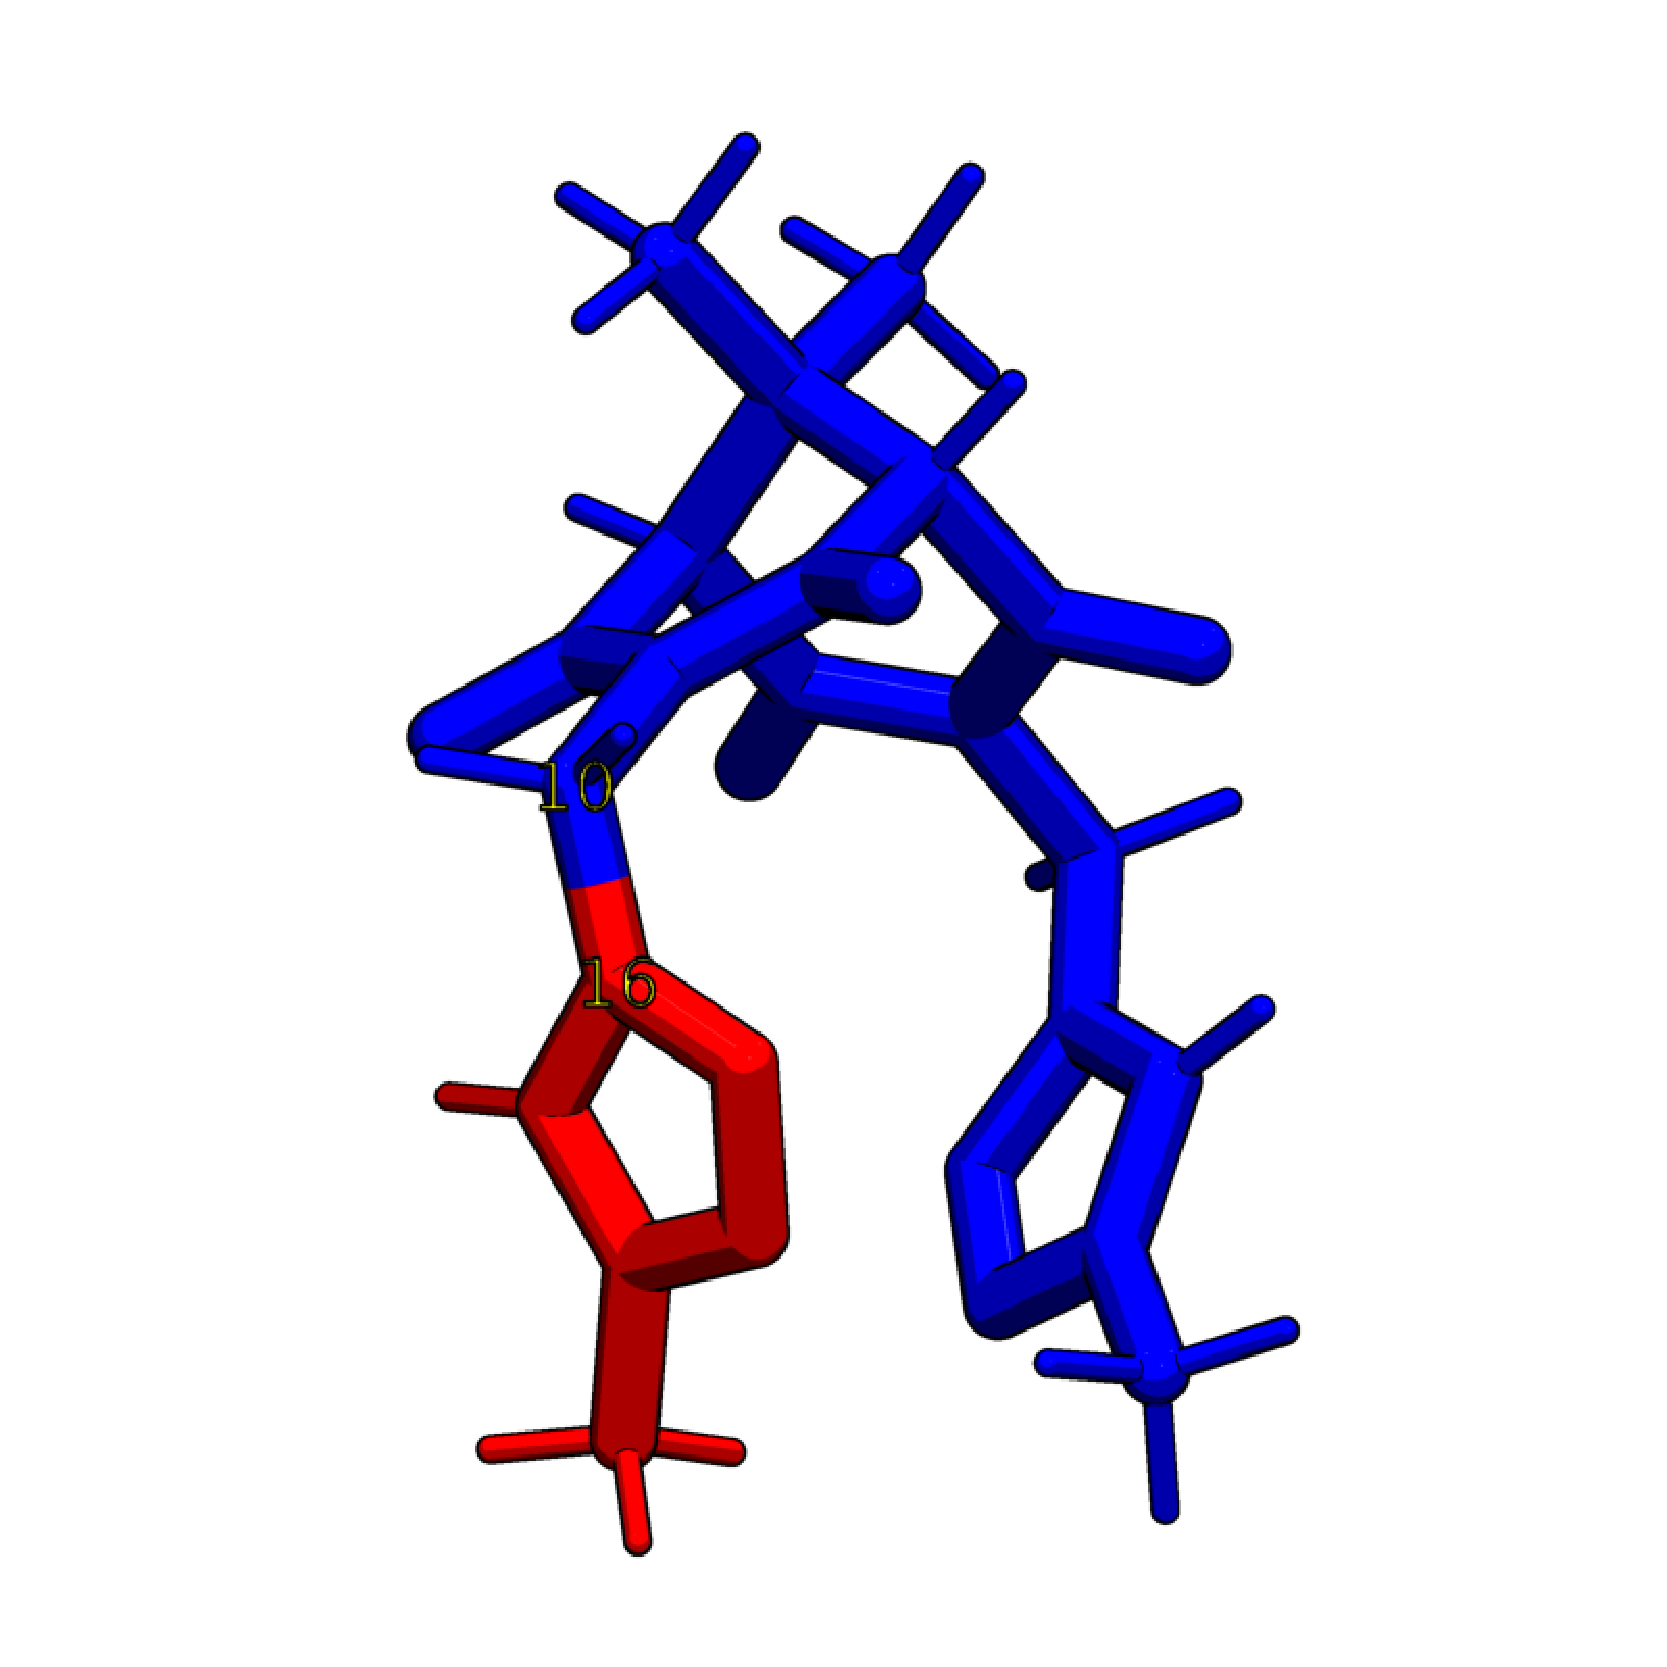
\includegraphics[width=0.5\textwidth]{./img/template_rotate_100}
  \caption{}
	\label{fig:template_rotate}
\end{figure}

Общая идея в том, чтобы разбить молекулу на две компоненты связности: красную (A) и синюю (B), затем провращать все атомы из компоненты А.


\end{document}
